\documentclass[11pt,oneside,openany]{book}
\usepackage{zlc_frontend_notes}

\begin{document}
\frontmatter
\zlctitlepage{原版 2D\_rearrangement notebook 详细教程}{逐 cell 解释、函数原理、Verilog 时序与同步风险}{PythonCamDemo / address\_switch 中性原子 2D 重排流程解析}{2026-05-31}
\tableofcontents
\cleardoublepage
\mainmatter


\chapter{阅读方式}
\section{这份教程讲什么}
这份教程只针对原版 \filepath{PythonCamDemo/2D_rearrangement.ipynb}。它不是重构代码说明，而是把原 notebook 按真实实验语义拆开：每个 cell 在做什么、每个函数的输入输出是什么、背后的物理和算法原理是什么、它怎样依赖 \filepath{address_switch} 的 Verilog 时序，以及我在阅读后发现的潜在时序问题、可能后果和修复办法。

这份 notebook 很大，里面同时存在正式流程、校准流程、移动测试、参数扫描、临时调试和过期输出。最重要的阅读原则是：\tfocus{不要把 notebook 输出等同于从上到下重新运行的结果}。有些 cell 的输出明显来自旧版本函数或非线性执行顺序；真正做实验时，应该 restart kernel 后只运行当前流程需要的 cell，并把函数定义固定下来。

\begin{figure}[htbp]
  \centering
  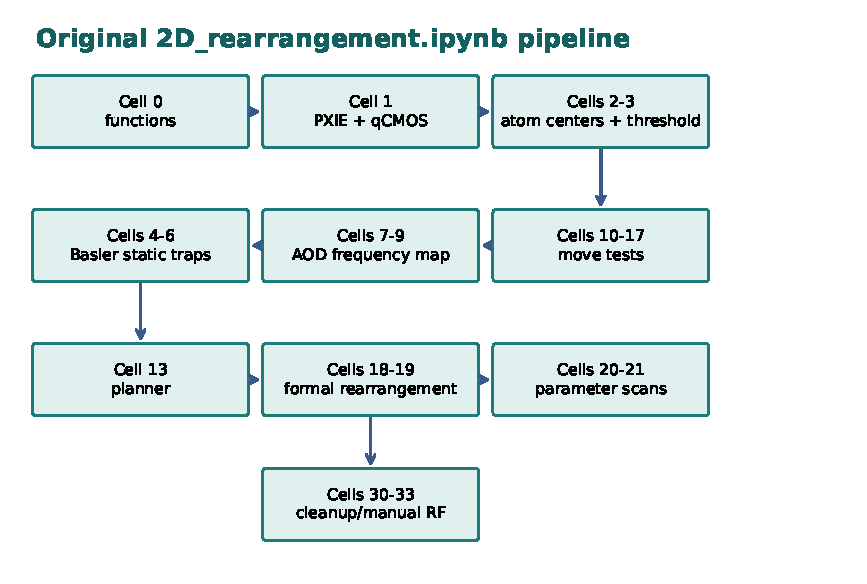
\includegraphics[width=0.96\textwidth]{assets/notebook_pipeline.pdf}
  \caption{原版 notebook 的功能块：先定义函数和连接硬件，再做 qCMOS/atom center/threshold 校准、Basler 静态阱校准、AOD 频率映射、移动测试、正式重排和参数扫描。}
\end{figure}

\section{这个 notebook 的核心实验合同}
原版流程隐含了一个很强的实验合同：
\begin{enumerate}
  \item FPGA 或其它时序硬件负责 MOT/PGC/probe/pushout/readout 等 TTL 序列，并向相机提供外触发边沿。
  \item Python 负责在相机已经外触发模式下等待图像，得到 before 图。
  \item Python 用 before 图判别哪些 site 有原子。
  \item planner 把当前 occupancy 和目标 target 变成若干条 site path。
  \item PXIE/AOD 按 path 移动原子，并把多余原子 move off。
  \item Python 再等待 after 图，统计 target fill rate 和 move success rate。
\end{enumerate}

问题在于，原版代码没有把这个合同显式写成一个同步协议。Python 在等相机，FPGA 在跑时序，PXIE 在移动原子，但三者之间没有一个统一的 shot transaction。只要其中一个环节晚一点、早一点、错过一个 trigger，before/after 图就可能不属于同一次实验循环。

\chapter{Cell-by-cell 教程}
\section{Cell 0: 函数定义总入口}
Cell 0 是整个 notebook 的函数库。它先 import DCAM、Basler、PXIE、OpenCV、SciPy 和 Matplotlib，然后在 notebook 内部重新定义 qCMOS、PXIE move、图像分析和画图函数。它包含的核心函数是：

\begin{description}
  \item[\pyapi{qCMOS_init}] 初始化 Hamamatsu qCMOS，设置外部触发、正沿触发、曝光时间、读出速度和硬件 ROI。
  \item[\pyapi{qCMOS_EXTERNAL_ra}] 单帧外触发等待，原意是“重排前/后拍一张图”。
  \item[\pyapi{qCMOS_EXTERNAL_detect}] 单帧或多帧外触发等待，\pyapi{buf_alloc > 1} 时返回 list，用于批量保存 loading 图。
  \item[\pyapi{qCMOS_end}] 释放 buffer、关闭 device、uninit DCAM API。
  \item[\pyapi{move_caculate}] 根据 AOD 起止频率计算两轴 ramp 的加速度、amplitude step 和累计 section。
  \item[\pyapi{move_atom}] 把 site path 变成 PXIE RA 参数并执行两轴移动。
  \item[\pyapi{moveoff_atom}] 把多余 atom 沿阵列外侧丢掉。
  \item[\pyapi{calculate_average_image}] 从 TIFF 文件夹读取多张 qCMOS 图，求平均图并返回所有 frame。
  \item[\pyapi{find_centers}] 用 Otsu threshold 和连通域找 trap/atom center，并按蛇形顺序排序。
  \item[\pyapi{threshold_calculate}] 对所有 site 的 3x3 ROI counts 做双高斯拟合，得到一个全局阈值。
  \item[\pyapi{identify_atom}] 对单张图按 center 和 threshold 判别 occupancy。
  \item[\pyapi{plot_rearrangement}] 显示 before/after 图，并标注被识别到的 atom site。
\end{description}

\begin{notebox}[重要现象]
Cell 0 中的函数会覆盖从 \filepath{pxie_control.py} 或其它模块 import 进来的同名函数。后面 Cell 10、Cell 11 的输出看起来来自旧版本 \pyapi{move_caculate(begin,end,...)}，但当前 Cell 0/12 中的 \pyapi{move_caculate} 接口是 \pyapi{move_caculate(frequency_AOD, path, ...)}。这说明 notebook 中存在旧输出或非线性执行顺序。教程后面会把这类 cell 归为调试/历史 cell。
\end{notebox}

\section{Cell 1: 连接 PXIE 和 qCMOS}
Cell 1 是硬件连接 cell：
\begin{codeblock}[Python]
card_id = 0x1A0000
pxie = pxie_set()
pxie.setParams(card_id, 0, 0, 9)
ra_openresult = pxie_open(pxie, card_id)

frequency_AOD = np.load("freq.npy")
FRAMES_PER_GROUP = 3
CROP_ROI = (1648, 64, 1144, 64)
dcam = qCMOS_init(exposure_time=0.02, readout_speed=1, roi=CROP_ROI)
\end{codeblock}

\pyapi{card_id} 是 PXIE 板卡 ID。这里的 \pyapi{0x1A0000} 与旧注释中的 \pyapi{0x170000} 不一致，所以真正实验前必须确认是哪张卡。 \pyapi{pxie.setParams(card_id, 0, 0, 9)} 设置 DLL/板卡的基础参数；\pyapi{pxie_open} 负责打开板卡并初始化工作模式。 \pyapi{frequency_AOD} 从 \filepath{freq.npy} 载入每个 site 对应的两轴 RF 频率。

\pyapi{CROP_ROI = (x, width, y, height)} 是 qCMOS 硬件 ROI。DCAM subarray 通常要求位置和尺寸满足硬件步进约束，这里注释写的是 4 的倍数。这个 ROI 不是 atom ROI；它只是相机读出的硬件裁剪区域。后面的 \pyapi{identify_atom} 还会在裁剪图上围绕每个 site center 做 3x3 ROI。

\section{Cell 2: 拍 100 张 loading 图并保存}
Cell 2 调用：
\begin{codeblock}[Python]
img_test = qCMOS_EXTERNAL_detect(dcam, buf_alloc=100, timeout_millisec=10000)
\end{codeblock}
当 \pyapi{buf_alloc=100} 时，相机进入 sequence capture。Python 逐帧等待外部 trigger，读出 100 张图，然后保存成 \filepath{Image1_1.tif}、\filepath{Image1_2.tif} 这样的文件。这个 cell 的目标是为 atom center 和 threshold 校准提供统计数据。

这里的物理含义是：外部时序需要连续产生足够多次 probe/readout 触发；每次触发之后相机曝光并读出一张 loading 图。若 FPGA 的 \pyapi{cycle_counts} 小于 100，或相机 trigger 线没有真正接到 qCMOS，代码会在某一帧 timeout。

\section{Cell 3: 求平均图、找 atom center、拟合阈值}
Cell 3 先读回 Cell 2 保存的 TIFF：
\begin{codeblock}[Python]
atom_image, all_frames = calculate_average_image(data_path, file_prefix)
atom_image = normalize_to_uint8(atom_image)
atom_centerlist = find_centers(atom_image, trap_numx=7, trap_numy=5, ...)
threshold = threshold_calculate(all_frames, atom_centerlist, plot=True)
\end{codeblock}

\pyapi{calculate_average_image} 的作用是把多张 loading 图叠加平均，得到更稳定的 atom/fluorescence 空间分布。它同时返回 \pyapi{all_frames}，用于后续 threshold 统计。

\pyapi{find_centers} 在平均图上做 Otsu 二值化。如果连通域数量少于 \pyapi{trap_numx * trap_numy + 1}，它会逐步降低 threshold 直到找到足够多的 bright blobs。找到连通域后，它不直接用质心，而是在每个连通域内部找最亮像素附近的位置作为 center。最后按 \pyapi{column_direction} 和 \pyapi{row_direction} 做蛇形排序。

\pyapi{threshold_calculate} 对每张 frame、每个 center 的 3x3 pixel sum 做直方图，然后用双高斯拟合暗态/亮态。两个峰之间拟合曲线的谷底作为 threshold。这个 threshold 是全局单值，不是每个 site 一个值。

\begin{notebox}[潜在误差]
如果不同 site 的荧光强度差别很大，全局 threshold 会让亮 site 的暗态和暗 site 的亮态混在一起，导致特定 site 系统性误判。更稳的做法是为每个 site 单独拟合 threshold，并把 threshold 与 center、ROI radius 和采集日期一起保存。
\end{notebox}

\section{Cell 4: Basler 相机初始化}
Cell 4 定义 \pyapi{camera_initialize(id)}，用 Basler pylon API 枚举相机并打开指定编号的相机。这里把 exposure 先设成 20，随后 Cell 5 会拉长曝光来拍静态阱。

Basler 在这个 notebook 中不是 atom detection 相机，而是用于看 SLM/static trap 和 AOD spot 的校准相机。它帮助把“图像上的静态阱位置”与“AOD RF 频率”对应起来。

\section{Cell 5: 拍 SLM/static trap center}
Cell 5 先把 PXIE 两轴 RF 关掉：
\begin{codeblock}[Python]
pxie.ssb_param_set(card_id, 0, 0, 0, 0, 0, 0)
pxie.ssb_param_set(card_id, 1, 0, 0, 0, 0, 0)
\end{codeblock}
然后用 Basler 长曝光拍静态阱，crop、transpose，再调用 \pyapi{find_centers} 得到 \pyapi{trap_centerlist}。这里 \pyapi{trap_centerlist} 是静态目标阵列在 Basler 图像上的坐标，不等同于 qCMOS 上的 \pyapi{atom_centerlist}。

\section{Cell 6: 单个 AOD spot 检查}
Cell 6 用 \pyapi{start_site = 10} 取 \pyapi{frequency_AOD[start_site]}，让 AOD 打出单个 spot，并用 Basler 看它是否落在预期位置。这是 auto-match 前的 sanity check：如果这里已经看不到 spot，后续梯度搜索会失败。

\section{Cell 7: 自动校准 AOD 频率映射}
Cell 7 定义 \pyapi{auto_match}。它对每个 static trap center 做一个频率优化：
\begin{enumerate}
  \item 从 \pyapi{[96 MHz, 96 MHz]} 或旧 \filepath{freq.npy} 中的频率出发。
  \item 把当前两轴频率写到 PXIE SSB。
  \item Basler 拍图并找当前 AOD spot center。
  \item 计算当前 spot 与目标 static trap center 的距离。
  \item 分别给 f0 和 f1 加一个小的 \pyapi{frequency_step}，拍两张图估算距离函数梯度。
  \item 用 Adam 风格的一阶/二阶动量更新频率。
  \item 距离小于 4 像素时认为收敛，保存该 site 的频率。
\end{enumerate}

这个 cell 的原理是把光学系统当成一个局部连续映射：
\[
  (f_0, f_1) \mapsto (x_\mathrm{AOD}, y_\mathrm{AOD}).
\]
优化目标是最小化 \(\|(x,y)-(x_\mathrm{target},y_\mathrm{target})\|^2\)。这里没有显式拟合 Jacobian，而是用有限差分估计梯度。

\begin{notebox}[潜在风险]
\pyapi{auto_match} 中多处使用 \pyapi{np.uint}。如果梯度更新让频率低于 0 或超出硬件范围，无符号整数会 wrap，频率会跳到巨大值。修复办法是：优化过程全程使用 Python \pyapi{int} 或 \pyapi{float}，每次写硬件前 clamp 到安全频率范围，最后保存时再转成整数。
\end{notebox}

\section{Cell 8: AOD 频率网格拟合}
Cell 8 把 Cell 7 得到的 \pyapi{frequency_AOD_basler} 转成 MHz，并用一个四参数模型拟合规则网格：
\[
  \mathbf f = s R(\theta)(\mathbf n-\bar{\mathbf n}) + (t_x,t_y).
\]
这里 \(\mathbf n\) 是人为构造的 7x5 交错逻辑网格，\(s\) 是频率间隔，\(\theta\) 是小旋转，\((t_x,t_y)\) 是中心频率。拟合后得到一个更平滑的 \pyapi{frequency_AOD}，保存回 \filepath{freq.npy}。

这个 cell 的意义是把逐点优化得到的 noisy frequency map 投影到规则模型上。好处是减少局部拍照误差；风险是如果真实频率网格有畸变、SLM static trap 不规则或排序错了，规则拟合会把真实误差平均掉，导致个别 site move 系统性偏移。

\section{Cell 9: 对比频率表}
Cell 9 主要是画图比较 \pyapi{frequency_AOD} 和 \pyapi{frequency_AOD1}。它不是正式流程的一部分，但非常适合作为频率映射 sanity check：检查点序是否蛇形、x/y 方向是否反了、拟合前后是否有异常跳点。

\section{Cells 10-12: PXIE move 测试}
Cells 10 和 11 是早期手写 PXIE RA 参数测试：设置起点 SSB、手动分配 \pyapi{speed/step/section} 数组、调用 \pyapi{ra_param_set}、\pyapi{ra_run}，然后拍 after 图。它们的输出很可能来自旧版 \pyapi{move_caculate}，不建议直接作为当前 notebook 的可复现实验流程。

Cell 12 重新定义了更完整的 \pyapi{move_caculate}、\pyapi{move_atom}、\pyapi{move_caculate_frequency} 和 \pyapi{moveoff_atom}，并打印从 site 0 到 site 1 的 ramp 参数。它更接近正式重排调用的版本。

\begin{figure}[htbp]
  \centering
  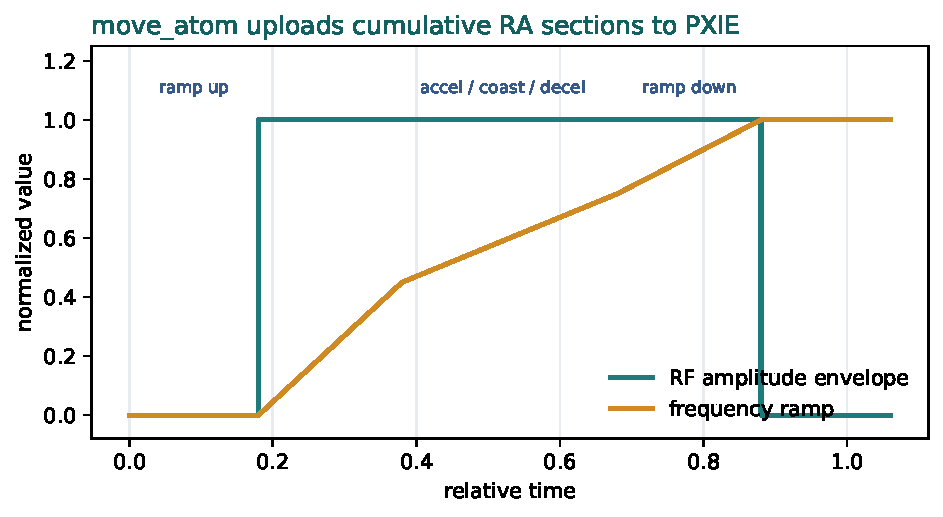
\includegraphics[width=0.88\textwidth]{assets/pxie_move_profile.pdf}
  \caption{\pyapi{move_atom} 的概念：先在起始 site 打开 RF amplitude，再用 RA segment 做频率 ramp，最后 ramp down。代码上传给 PXIE 的 section 是累计 tick。}
\end{figure}

\section{Cell 13: planner 算法测试}
Cell 13 是重排算法的核心测试。它先定义一个 35-site 的 \pyapi{atom_centerlist} 和目标 target：
\begin{codeblock}[Python]
target = [8, 6, 7, 12, 11, 18, 16, 17, 22, 21, 28, 26, 27]
\end{codeblock}

然后定义三类函数：
\begin{description}
  \item[\pyapi{build_neighbor_graph}] 根据 site 像素坐标和 \pyapi{max_dist=11} 建邻接图。距离小于阈值的 site 被认为可以一步移动。
  \item[\pyapi{find_graph_path}] 用 Dijkstra-like 优先队列找从起点到目标的路径。经过已占据 site 时增加 15 的 penalty，所以算法会优先绕开原子，但必要时允许“推挤”。
  \item[\pyapi{compress_algorithm}] 先用 Hungarian matching 把 stray atoms 分配给 empty targets，再按目标离中心距离排序，逐个找路径并更新 occupancy。路径上有多个 occupied site 时，从路径末端往前推，形成 cascade pushing。
\end{description}

\pyapi{compress_algorithm} 返回：
\begin{itemize}
  \item \pyapi{move_step}：每个 atom 的移动段，例如 \pyapi{[[24, 23], [23, 22]]}。
  \item \pyapi{start_positions}：被选来移动的初始 atom site。
  \item \pyapi{target_positions}：本次移动最终填到的目标 site。
\end{itemize}

它的核心思想是：宏观上用 Hungarian 算法减少总距离，局部上用 occupancy-aware graph path 避免碰撞。当前实现的 collision model 仍然比较粗糙：它只用 penalty 表示被占据 site，不真的模拟移动过程中两个 atom 同时出现在同一个 trap 的动力学约束。因此它适合作为实验 planner 雏形，但不应该把它当成已完成的硬件安全验证。


\begin{figure}[htbp]
  \centering
  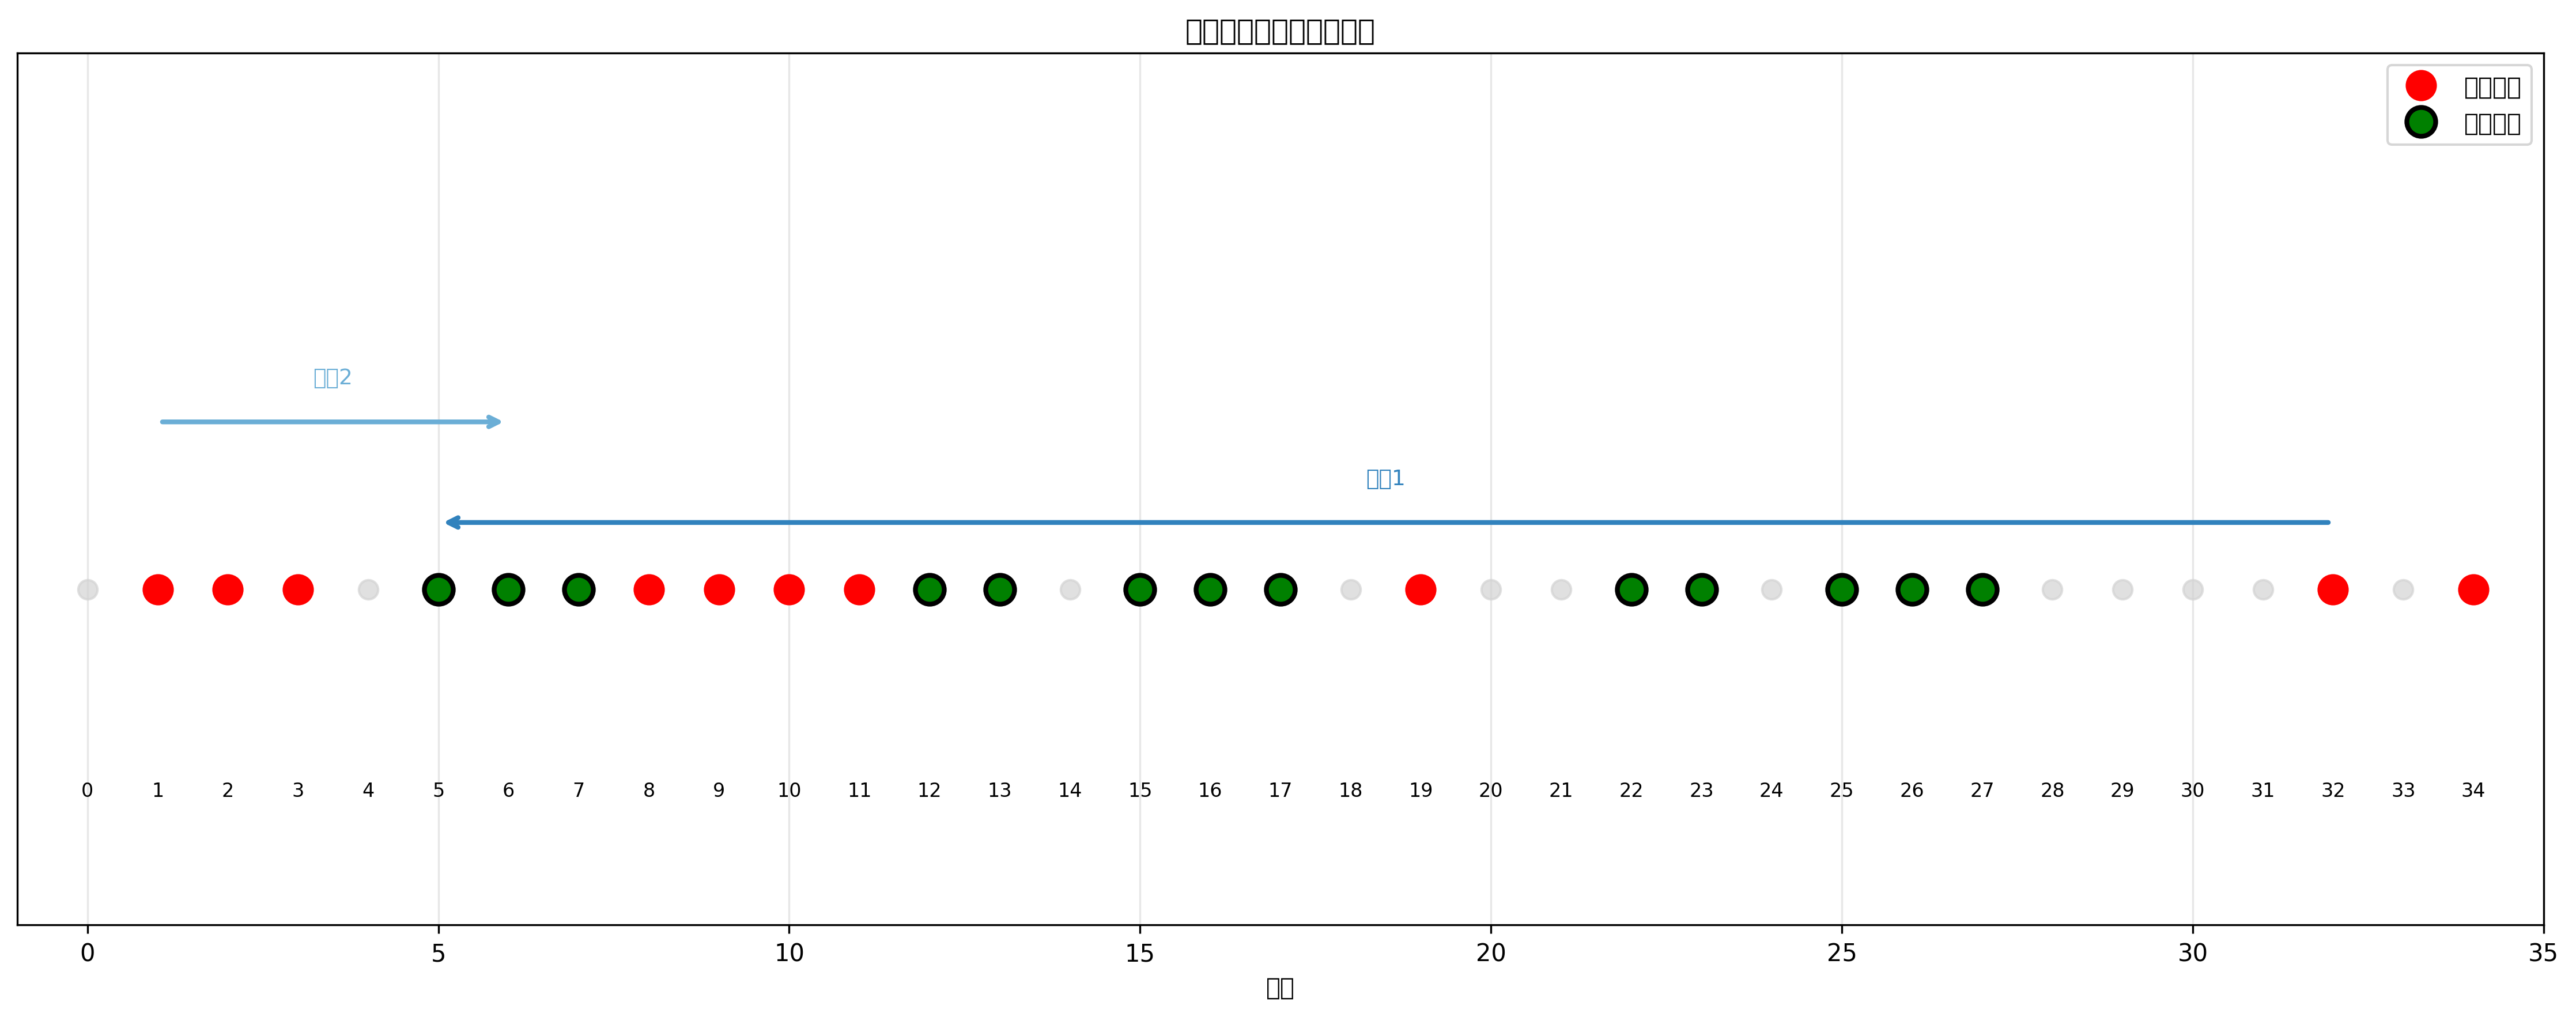
\includegraphics[width=0.88\textwidth]{assets/atom_movement.png}
  \caption{原始 notebook 附带的 atom movement 图。它展示的是完整链条的结果：before 图像判别、planner 给出路径、PXIE 执行 move、after 图像重新判别。}
\end{figure}


\begin{figure}[htbp]
  \centering
  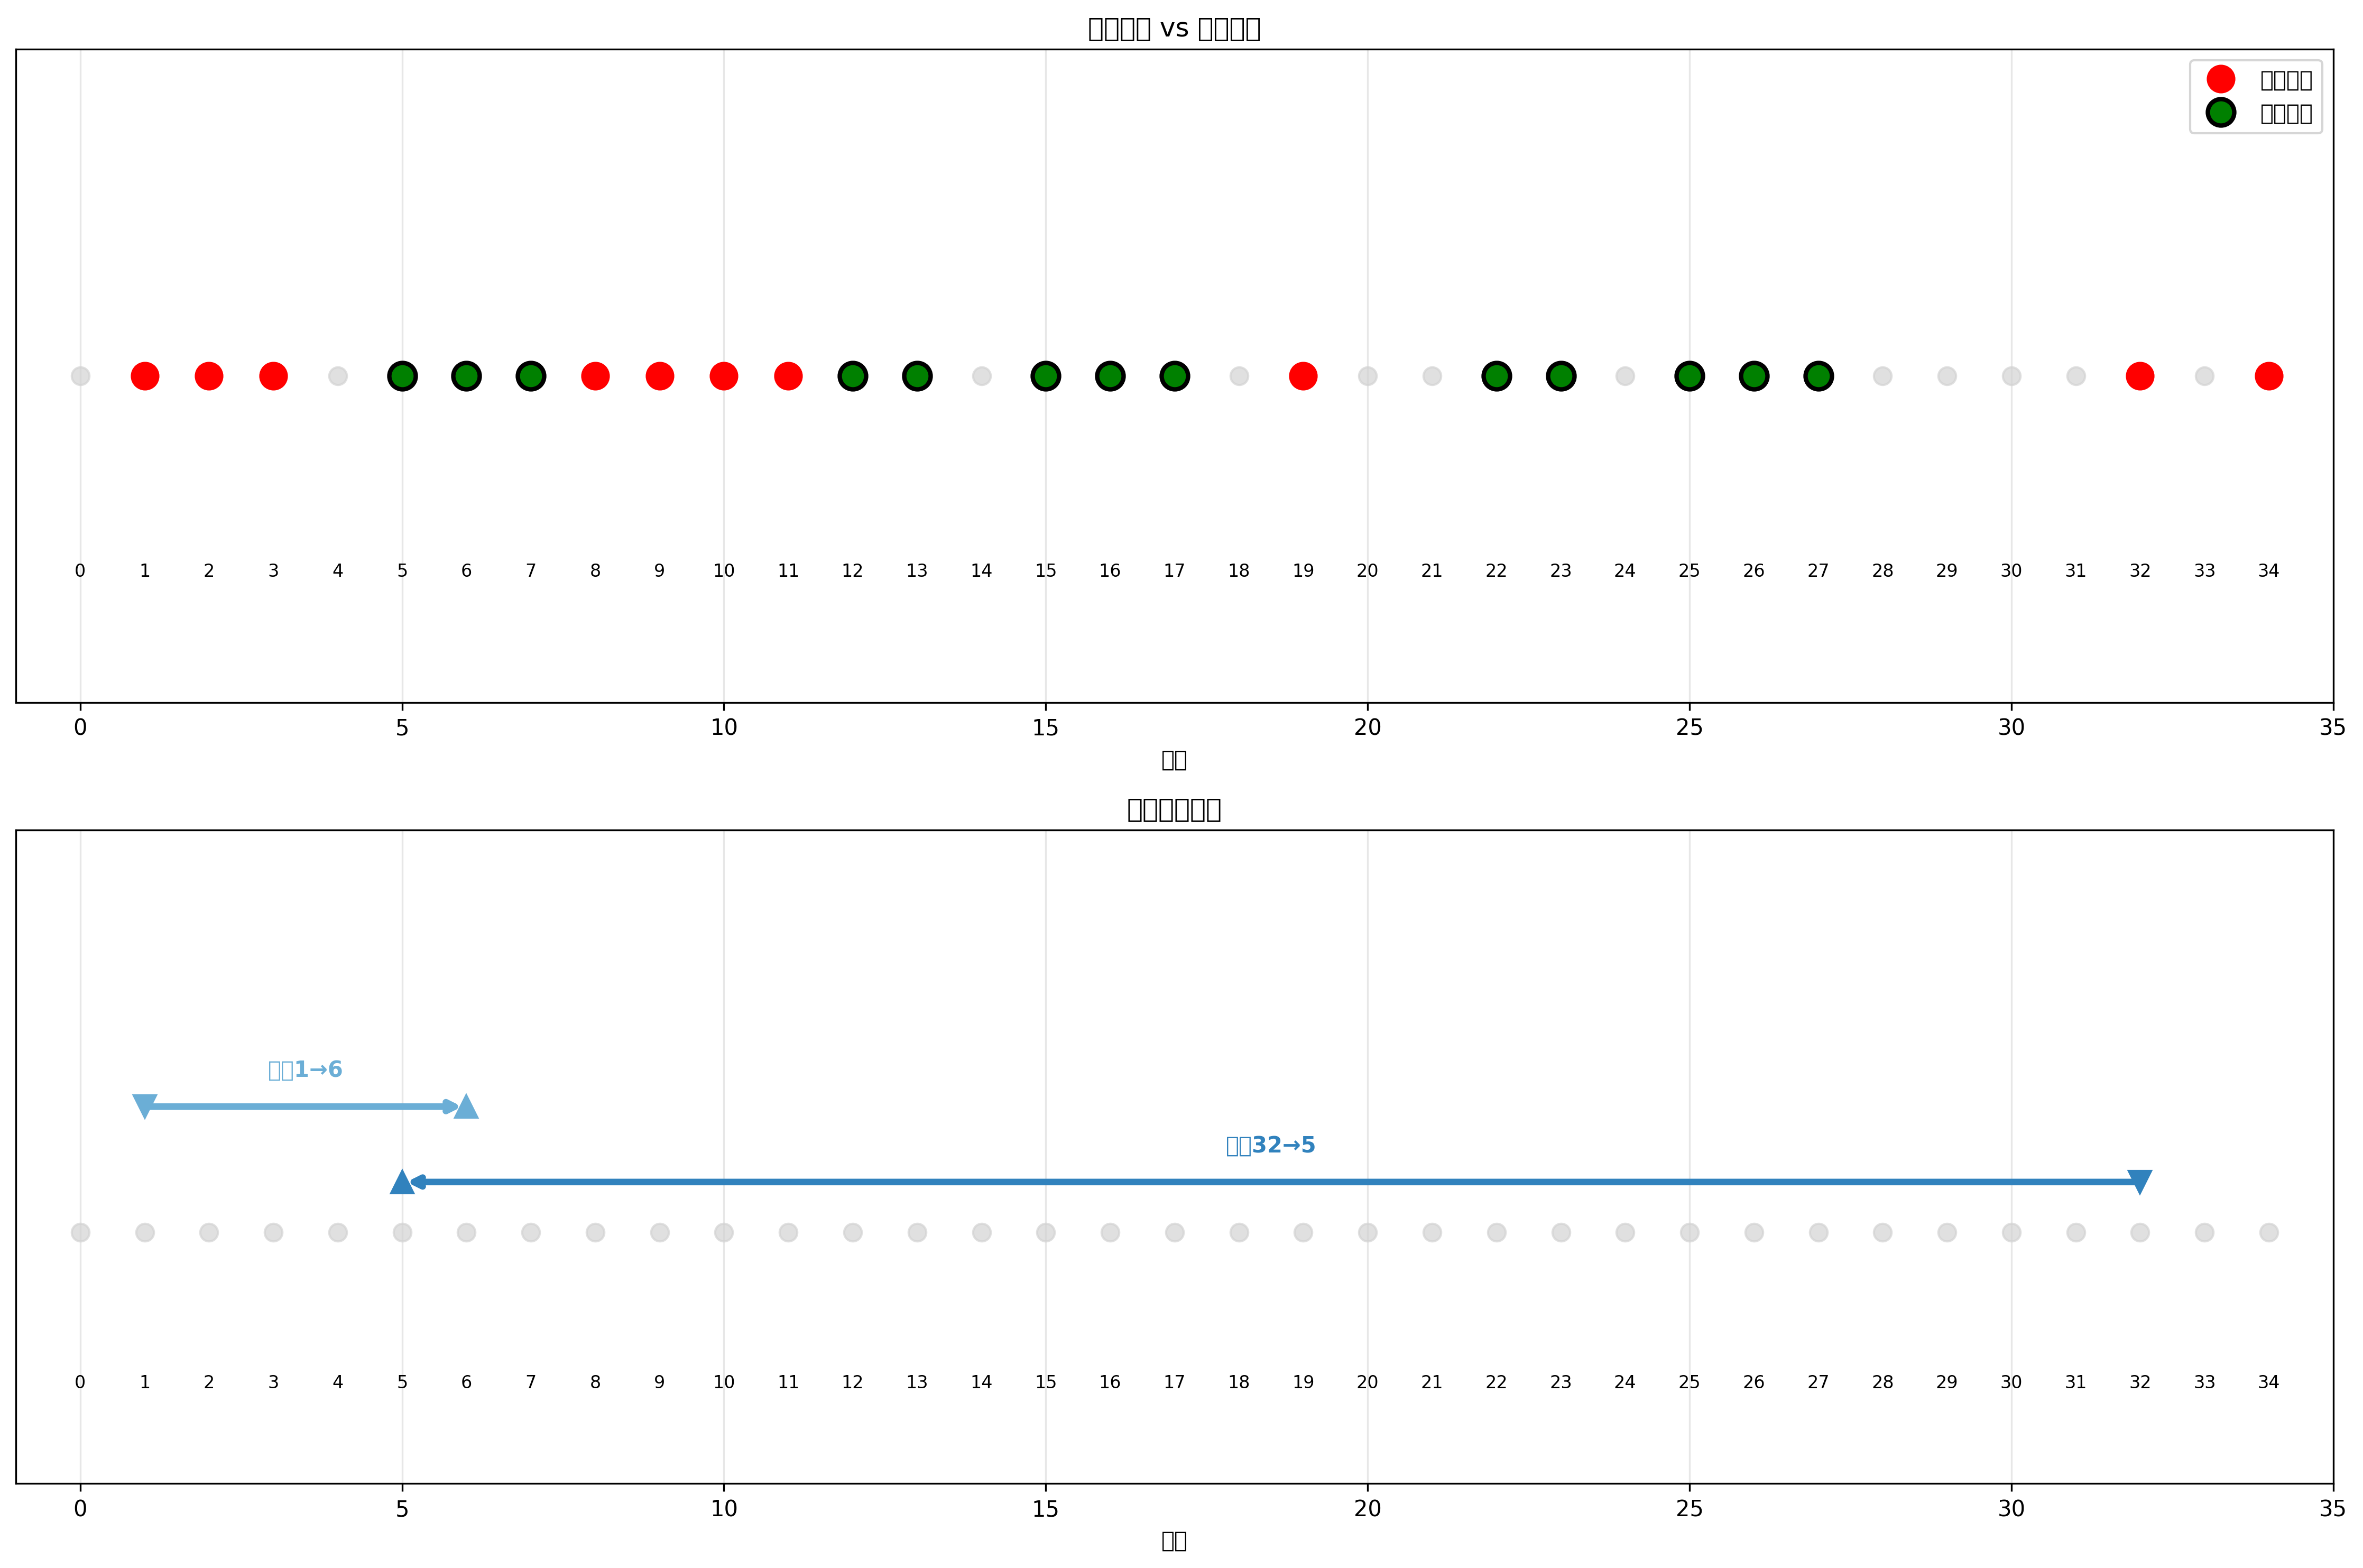
\includegraphics[width=0.88\textwidth]{assets/atom_movement_enhanced.png}
  \caption{增强版结果图。教程中把这类图当成验证终点：不仅要看最终 target 是否填满，还要能追溯每条路径、每个 threshold 和每段 PXIE ramp。}
\end{figure}


\section{Cell 14: eta 和单步路径测试}
Cell 14 重新设置 \pyapi{pxie.setParams}，定义 \pyapi{atom_path = [[0,4]]}，调用 \pyapi{move_atom} 测试长一步移动。这里主要是在调 \pyapi{a}、\pyapi{time_a} 和内部 \(\eta\) 常数。

\(\eta\) 的角色是把频率差和 ramp tick 联系起来。长距离使用三段式：加速、匀速、减速；短距离使用两段式：加速、减速。分界条件大致来自
\[
  \Delta f_\mathrm{threshold} \sim \frac{t_a^2}{\eta}.
\]
这个模型的物理含义是 RF frequency chirp 不能太快，否则 atom 在移动光镊中会被激发或丢失；也不能太慢，否则重排时间长，寿命损失增加。

\section{Cells 15-17: move off 和固定方向测试}
Cell 15 测试 \pyapi{moveoff_atom}：先拍 before，然后把所有或多余原子沿阵列外侧移走，再拍 after。Cells 16 和 17 手写固定路径测试“向上移动一格”和“向左移动一格”。这些 cell 的目的不是统计最终成功率，而是验证：
\begin{itemize}
  \item \pyapi{frequency_AOD} 的方向是否和 site index 对齐。
  \item \pyapi{moveoff_atom} 是否真的把 atom 移出 ROI。
  \item \pyapi{move_atom} 的 ramp 参数是否太快或太慢。
  \item before/after 图是否来自同一个时序窗口。
\end{itemize}

\section{Cell 18: 正式重排程序}
Cell 18 是最重要的正式流程：
\begin{enumerate}
  \item 设置 target、保存目录、循环次数和 PXIE ramp 参数。
  \item 每轮先调用 \pyapi{qCMOS_EXTERNAL_ra} 等 before 图。
  \item 用 \pyapi{identify_atom} 得到当前 loaded atoms。
  \item 用 \pyapi{compress_algorithm} 得到 \pyapi{array_path}、\pyapi{atom_choose}、\pyapi{move_target}。
  \item 对每条 path 调 \pyapi{move_atom}。
  \item 把 channel 1 设置到 \pyapi{100000, amp=0}，相当于试图关掉或移除某一路 RF。
  \item 对 stray atoms 调 \pyapi{moveoff_atom}。
  \item 再关一次 channel 1。
  \item 调 \pyapi{qCMOS_EXTERNAL_detect} 等 after 图。
  \item 统计 target fill rate、move success rate 和每个 target 的成功率。
\end{enumerate}

这个 cell 的统计有两个概念：
\begin{description}
  \item[target fill rate] after 图中 target set 被占据的比例，反映最终阵列填充效果。
  \item[move success rate] planner 认为需要移动到的 \pyapi{move_target} 中，有多少在 after 图里真的有 atom。
\end{description}

\begin{notebox}[正式流程的同步弱点]
\pyapi{t1 - t0 < 1} 被用来判断记录是否有效，但它只说明 Python 从 before 后到 after 后用了不到 1 秒，不能证明 before/after 属于同一个 FPGA shot，也不能证明 after 图发生在 PXIE move 完成之后。真正需要记录的是：camera armed time、FPGA trigger edge time、PXIE start/finish time 和 frame index。
\end{notebox}

\section{Cell 19: 重排加寿命对照}
Cell 19 在 Cell 18 的基础上加入对照组。实验组做重排，然后对照组只拍 before、等待与重排耗时近似相同的 \pyapi{ra_duration}、再拍 after。它想区分“移动失败”与“自然寿命损失”：
\begin{itemize}
  \item 如果重排成功率低，但自然存活率也低，问题可能主要是 lifetime 或 readout heating。
  \item 如果自然存活率高，但移动成功率低，问题更可能在 AOD move、frequency map 或 planner collision。
\end{itemize}

这个设计方向是对的，但原实现仍然受同一个 trigger 同步问题限制。对照组的 \pyapi{time.sleep(ra_duration)} 是 Python 侧延迟，不是 FPGA shot 中严格定义的等待。如果 FPGA 自己在循环，sleep 不会控制下一次 trigger 的相位。

\section{Cells 20-21: 参数扫描}
Cell 20 扫 \pyapi{frequency_AOD} 的二维 offset，得到每个 target 的 move success rate heatmap。它用于回答：频率表整体偏了多少时成功率最好。

Cell 21 扫 \pyapi{time_a}，得到总体 fill rate、move success rate 和每个 target 的热力图。它用于找移动速度折中：\pyapi{time_a} 太小，移动太快容易丢；\pyapi{time_a} 太大，移动太慢导致 lifetime 损失或 cycle 变长。

这两个扫描都有一个共同风险：如果底层时序不同步，heatmap 可能把 trigger 抖动、丢帧、跨 cycle 捕获误当成 AOD 参数效应。扫描前必须先用示波器或记录 trace 确认 before/after trigger 与 PXIE move 的相对时间稳定。

\section{Cells 22-29: 临时调试区}
Cells 22-25 是临时检查变量和显示图像。Cell 24 甚至有 \pyapi{ValueError} 输出，说明它不是稳定流程的一部分。

Cell 26 测 AOD static trap 位置。Cell 27 测单阱移动。Cells 28-29 是重排测试的单长步和三步版本。这些 cell 应该在教程中视为“实验者的 scratch pad”：有价值的是里面暴露出的参数和现象，不应该直接复制到正式实验脚本。

\section{Cells 30-33: 关闭与手动 RF 控制}
Cell 30 调 \pyapi{qCMOS_end(dcam)} 释放相机。Cell 31 调 \pyapi{pxie.Card_Close(card_id)}，但 notebook 输出中有 \pyapi{OSError}，说明 DLL close 或 card handle 状态可能不一致。更稳的做法是在打开/关闭设备时维护一个明确状态，并在 close 前检查 card 是否已经 open。

Cells 32-33 是手动 RF/SLM/AOM 控制。它们直接设置 \pyapi{ssb_param_set}，用于手动调频率、打开/关闭 AOD 和 SLM AOM。这里出现 \pyapi{card_id_AOM}，但它不是在 Cell 1 中定义的正式变量；因此这些 cell 依赖外部 notebook 状态或旧环境。

\chapter{函数原理详解}
\section{qCMOS 初始化和外触发}
\pyapi{qCMOS_init} 做的事很直接：
\begin{enumerate}
  \item \pyapi{Dcamapi.init()} 初始化 DCAM API。
  \item \pyapi{Dcam(0).dev_open()} 打开第一台相机。
  \item 设置 \pyapi{EXPOSURETIME}、\pyapi{TRIGGERSOURCE=EXTERNAL}、\pyapi{TRIGGERACTIVE=EDGE}、\pyapi{TRIGGERPOLARITY=POSITIVE} 和 \pyapi{READOUTSPEED}。
  \item 如果给了 ROI，则设置 \pyapi{SUBARRAYHPOS/HSIZE/VPOS/VSIZE} 并开启 \pyapi{SUBARRAYMODE}。
\end{enumerate}

它的实验含义是：相机不会自己拍照，必须等外部 TTL 正沿。Python 只是 arm camera 并等 frame ready。这里的关键不是 Python 何时调用 \pyapi{wait_capevent_frameready}，而是外部 TTL 边沿是否发生在相机已经 armed 之后。

\pyapi{qCMOS_EXTERNAL_ra} 和 \pyapi{qCMOS_EXTERNAL_detect} 的差别主要是名字和多帧支持。二者都应该在 timeout 后返回 \pyapi{None}，调用者必须检查。如果 after 图为 \pyapi{None} 还继续 \pyapi{identify_atom}，会造成异常或错误统计。

\section{center detection}
\pyapi{find_centers} 的重要步骤是：Otsu 二值化、连通域、按面积选最大 blobs、去掉距离太近的重复 blobs、把连通域 center 修正到最亮像素、蛇形排序。蛇形排序由 \pyapi{column_direction} 和 \pyapi{row_direction} 控制。

排序是整个重排里最危险的隐式约定之一。site index 同时连接了三件事：
\begin{itemize}
  \item qCMOS 图上的 \pyapi{atom_centerlist[index]}。
  \item AOD 频率表里的 \pyapi{frequency_AOD[index]}。
  \item planner 图中的 \pyapi{target} 和 \pyapi{array_path}。
\end{itemize}
只要一个排序方向反了，planner 会以为自己在移动 site 8，PXIE 实际却驱动另一个光镊位置。

\section{threshold fitting}
\pyapi{threshold_calculate} 把所有 frame 和所有 site 的 3x3 ROI sum 混在一起做一个总直方图，然后 fit 双高斯。它适合快速估计全局 loading threshold，但不适合作为最终高保真判别：
\begin{itemize}
  \item 每个 site 亮度不同会拉宽亮态峰。
  \item 相机背景不均匀会拉宽暗态峰。
  \item 如果 loading rate 太低或太高，双峰中一个峰样本不足，fit 会不稳定。
  \item fit 失败时退回 mean threshold，这在 bimodal 判别中通常不是最优 cut。
\end{itemize}

修法是改成 per-site threshold，并保存每个 site 的暗态均值、亮态均值、sigma、fidelity、样本量和 fit 状态。这样正式重排中可以知道哪几个 site 判别本来就差。

\section{PXIE move profile}
\pyapi{move_caculate} 以 site path 为输入，把每个相邻 site move 拆成两轴的频率 ramp。每轴独立计算自然耗时，再把短轴补一个等待段，让两轴同时结束。输出不是直接频率值，而是 PXIE RA 需要的：
\begin{itemize}
  \item \pyapi{speed0/speed1}：每段频率加速度或 chirp speed。
  \item \pyapi{step0/step1}：每段 amplitude step，ramp up/down 用它。
  \item \pyapi{section0/section1}：累计 tick，即每段结束的绝对 tick。
\end{itemize}

\pyapi{move_atom} 先设置起点 SSB：f0 channel amplitude 为 0，f1 channel amplitude 为 \pyapi{amp_max}。然后添加 ramp up、频率 move、ramp down，最后调用 \pyapi{ra_param_set} 上传 channel 0 和 channel 1，并分别 \pyapi{ra_run}。

\begin{notebox}[两轴同步风险]
\pyapi{move_atom} 最后依次调用 \pyapi{pxie.ra_run(card_id,0)} 和 \pyapi{pxie.ra_run(card_id,1)}。如果这两个调用不是硬件同步启动，两轴会有软件调用延迟。对于高速移动，几微秒的两轴相位差也可能让光镊轨迹偏离预期。若 DLL 支持双通道同步启动，应使用同步 run；否则至少用示波器或板卡 trace 测两轴起始延迟。
\end{notebox}

\section{move off}
\pyapi{moveoff_atom} 根据 \pyapi{discard_site < len_array/2} 判断向左还是向右丢。它只沿一条频率轴做 move，目的不是把 atom 移到另一个 site，而是把 atom 带到阵列外并 ramp down。

这里有两个细节。第一，margin 用 \pyapi{0.37} 倍阵列频率宽度，经验性很强，需要根据真实阵列大小和 AOD 可用带宽确认。第二，函数主要上传 channel 0 的 RA，channel 1 维持起始频率和 amplitude；后续 cell 用 \pyapi{ssb_param_set(card_id, 1, 0, 100000, 0, 0, 0)} 试图关掉 channel 1。这种“函数外补关”的方式容易漏掉，最好封装进 move off 函数内部。

\section{planner}
planner 的理论结构是两层：
\begin{enumerate}
  \item Assignment 层：把 stray atoms 和 empty targets 做 Hungarian matching，减少总移动距离。
  \item Routing 层：在邻接图中找 path，经过 occupied site 加 penalty，并用 cascade pushing 从路径末端往前移动，避免直接撞到已有 atom。
\end{enumerate}

这个设计很适合 2D array，因为它把“选哪个 atom 填哪个 target”和“怎么沿图移动”拆开了。缺点是它还没有把真实移动物理放进去：不同方向的 AOD move 成功率不同、长路径中间停顿会 heating、路径之间可能共享 site、移动顺序对最终 collision 有影响。这些都应该变成 planner cost 或 preflight，而不是靠 after 图事后发现。

\chapter{Verilog 对应关系}
\section{Python notebook 和 FPGA 的关系}
原 notebook 没有直接在 Python 中控制 \filepath{address_switch} 的 VIO 参数。实际实验应该是：Vivado/FPGA 已经烧录 \filepath{address_switch}，VIO 中设置好了 MOT/PGC/probe/pushout/readout 时序；Python 只负责 qCMOS 等外触发和 PXIE AOD move。

因此二者的耦合点只有几个 TTL/时间事实：
\begin{itemize}
  \item qCMOS 外触发线必须来自 FPGA 某个输出，例如 \pyapi{trig}、\pyapi{emCCD} 或另一路实际连接的 TTL。
  \item probe/readout TTL 必须覆盖 qCMOS 曝光窗口。
  \item before 图和 after 图必须属于同一个逻辑实验 transaction。
  \item PXIE move 必须发生在 before readout 后、after readout 前，且 FPGA 不能在 move 中途发出 after trigger。
\end{itemize}

\begin{figure}[htbp]
  \centering
  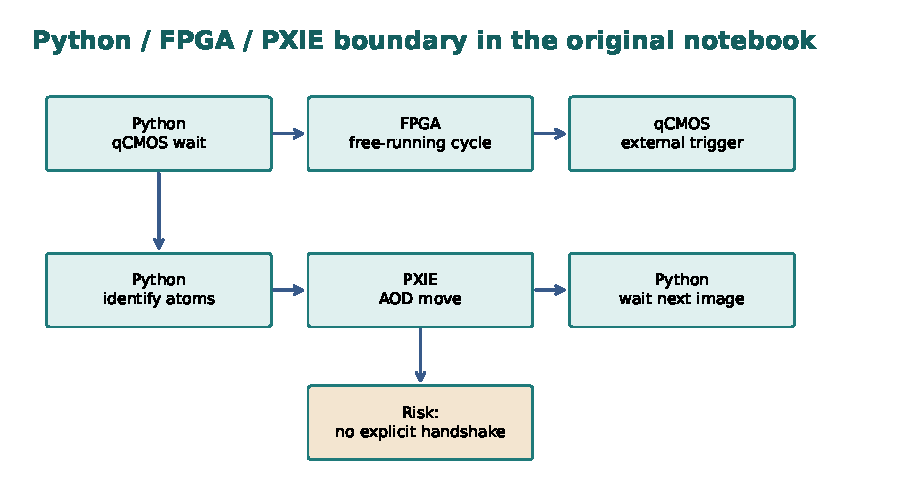
\includegraphics[width=0.95\textwidth]{assets/python_fpga_boundary.pdf}
  \caption{原版 notebook 的边界风险：Python、FPGA 和 PXIE 各自运行，但没有显式 handshake。}
\end{figure}

\section{main.v 做什么}
\filepath{main.v} 是顶层 module。它把物理端口列出来：\pyapi{cooling}、\pyapi{repump}、\pyapi{probe}、\pyapi{emCCD}、\pyapi{trap}、\pyapi{address}、\pyapi{trig}、\pyapi{pushout}、DA outputs 和 shutter outputs。然后实例化 \pyapi{vio_0}，把 \pyapi{probe_out0..47} 接到有名字的 wire，再传给 \pyapi{time_sequence}。

换句话说，\filepath{main.v} 主要是“VIO 参数桥”和“pin-level 顶层壳”。实验时你在 VIO 里改的 \pyapi{mot_lasting}、\pyapi{probe_waiting}、\pyapi{pulse_lasting}、\pyapi{cycle_counts}、\pyapi{probe_on} 等最终都进入 \filepath{time_sequence.v}。

\section{time-sequence.v 的运行方式}
\filepath{time_sequence.v} 有两个 always block。第一个 always block 维护 \pyapi{time_count}、\pyapi{cycle_time}、\pyapi{counts}、\pyapi{flag} 和 Ramsey 计数。只要 \pyapi{config_ready} 为 1，它就按 \pyapi{clk} 递增 \pyapi{time_count}；达到 \pyapi{cycle_time} 后回到 0；达到 \pyapi{cycle_counts} 后设置 \pyapi{flag}。

第二个 always block 产生 TTL/DA 输出。它有两种模式：
\begin{description}
  \item[debug 模式] \pyapi{debug=1} 时，VIO 的 \pyapi{cooling_on/probe_on/address_on/trap_on/...} 直接控制输出。这个模式适合手动对光、测 TTL cable、检查 shutter。
  \item[run 模式] \pyapi{debug=0} 且 \pyapi{config_ready=1} 时，用大量 \pyapi{if(time_count == ... )} 的累计时间条件切换输出。
\end{description}

\begin{figure}[htbp]
  \centering
  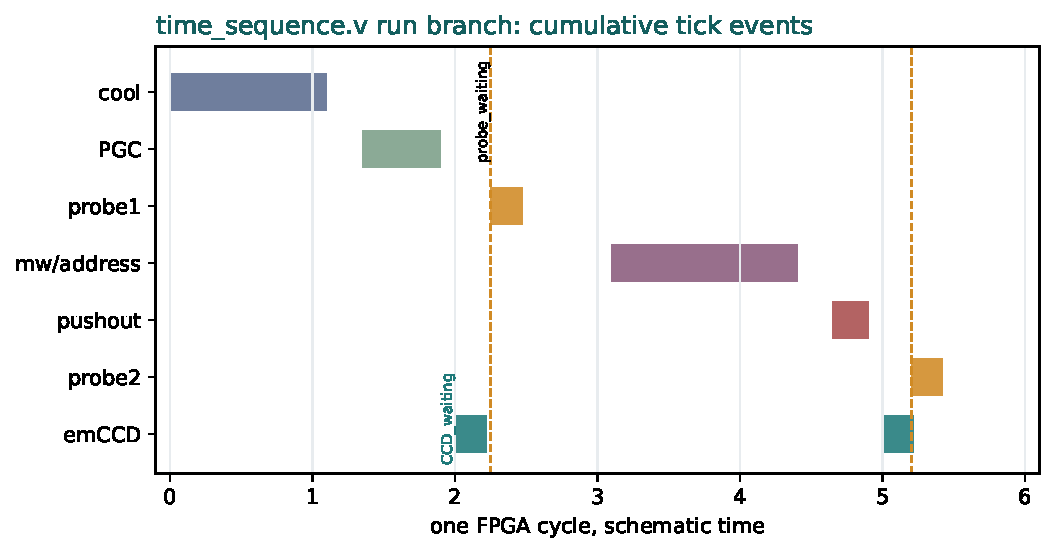
\includegraphics[width=0.95\textwidth]{assets/verilog_timeline.pdf}
  \caption{\filepath{time_sequence.v} run 分支的示意时间线。实际代码通过累计 tick 条件切换状态，而不是通过显式 phase state machine。}
\end{figure}

\section{和 qCMOS 相关的 Verilog 输出}
硬件 pin 约束中 \pyapi{trig} 在 R17，\pyapi{probe} 在 N15，\pyapi{emCCD} 在 M13。代码中：
\begin{itemize}
  \item debug 分支里，\pyapi{cooling_on} 会同时控制 \pyapi{cooling} 和 \pyapi{trig}。
  \item run 分支里，没有看到 \pyapi{trig <= ...} 的明确赋值。
  \item run 分支里 \pyapi{emCCD} 在 \pyapi{CCD_waiting} 和 \pyapi{CCD_waiting + pulse_lasting} 附近开关。
  \item run 分支里 \pyapi{probe} 在 \pyapi{probe_waiting} 和 \pyapi{probe_waiting + pulse_lasting} 附近开关。
\end{itemize}

这意味着：如果 qCMOS trigger cable 接在 \pyapi{trig}，run 模式下很可能没有正确 trigger；如果实际接在 \pyapi{emCCD}，那代码名会误导，而且 \pyapi{CCD_waiting} 与 \pyapi{probe_waiting} 必须严格对齐；如果实际接在 \pyapi{probe}，那相机触发与 probe 光同边沿，可能没有 trigger lead time。

\section{应该怎样操作原版 Verilog}
在不重写 Verilog 的前提下，比较安全的操作流程是：
\begin{enumerate}
  \item Vivado program FPGA，打开 VIO。
  \item 先置 \pyapi{config_ready=0}，确保 \pyapi{time_count/counts/flag} reset。
  \item 置 \pyapi{debug=1}，分别打开 \pyapi{probe_on}、\pyapi{trap_on}、\pyapi{cooling_on}、\pyapi{address_on}，用示波器确认每条 TTL 和 pin map。
  \item 确认 qCMOS 外触发线到底接在 \pyapi{trig}、\pyapi{emCCD} 还是其它输出，并在示波器上同时看 probe 和 trigger。
  \item 设置 run 参数：\pyapi{mot_lasting}、\pyapi{PGC_waiting}、\pyapi{PGC_lasting}、\pyapi{probe_waiting}、\pyapi{pulse_lasting}、\pyapi{pushout_waiting}、\pyapi{pushout_lasting}、\pyapi{cycle_counts} 等。
  \item 置 \pyapi{debug=0}，Python 先 arm qCMOS，再置 \pyapi{config_ready=1} 发起有限 cycle。
  \item cycle 结束后置 \pyapi{config_ready=0}，避免 FPGA 自己继续跑下一轮而 Python 还在处理上一轮。
\end{enumerate}

原 notebook 没有第 6-7 步的程序化 handshake，所以如果你现在是手动 VIO 让 FPGA 自由循环，Python 捕获到的图可能只是“下一次出现的 trigger”，而不是你以为的那一次 shot。

\chapter{潜在时序问题、后果和修复}
\section{问题 1: run 模式下 qCMOS trigger 不明确}
现象：\filepath{time_sequence.v} 中 \pyapi{trig} 只在 debug 分支由 \pyapi{cooling_on} 控制，run 分支没有明确 camera trigger pulse。

可能后果：
\begin{itemize}
  \item qCMOS 永远 timeout。
  \item qCMOS 偶尔被其它串扰或错误 TTL 触发，导致 before/after 图随机错位。
  \item debug 模式能触发，run 模式不能触发，造成“手动好用、正式实验不同步”。
\end{itemize}

修复：
\begin{itemize}
  \item 在 Verilog 中新增明确的 \pyapi{qcm_trigger} 或在 run 分支明确驱动 \pyapi{trig}。
  \item 每个 readout 只发一个正沿 trigger，宽度用参数 \pyapi{trigger_lasting} 控制。
  \item 用示波器同时看 \pyapi{trig}、\pyapi{probe}、qCMOS exposure out 或 frame valid。
  \item Python preflight 检查请求帧数等于 sequence 中 trigger 数。
\end{itemize}

\section{问题 2: camera waiting 和 probe waiting 混用}
run 分支中 probe 用 \pyapi{probe_waiting}，emCCD 用 \pyapi{CCD_waiting}。但是 \pyapi{cycle_time} 的总长度使用的是 \pyapi{probe_waiting} 和 \pyapi{pulse_lasting}，没有把 \pyapi{CCD_waiting} 明确纳入最后 cycle end 计算。

可能后果：
\begin{itemize}
  \item qCMOS trigger 早于 probe，曝光窗口里没有光。
  \item trigger 晚于 probe，曝光错过荧光。
  \item 如果 \pyapi{CCD_waiting > probe_waiting}，emCCD/off event 可能接近或超过 cycle end。
  \item 第一张图和第二张图使用不同等待变量，导致 before/after 时间间隔不等。
\end{itemize}

修复：
\begin{itemize}
  \item 定义显式事件时间：\pyapi{probe1_start}、\pyapi{cam1_trigger}、\pyapi{probe2_start}、\pyapi{cam2_trigger}。
  \item 用 \pyapi{camera_trigger_lead} 表示 trigger 比 probe 早多少 tick。
  \item \pyapi{cycle_time} 应该是所有 event end time 的最大值加 \pyapi{end_lasting}，不能手写漏掉 \pyapi{CCD_waiting}。
  \item 在 Python 生成 edge table 时做 validation：所有 trigger 都被 probe/exposure window 覆盖。
\end{itemize}

\section{问题 3: Python 等相机与 FPGA 自由循环没有 handshake}
原 notebook 中 \pyapi{img_before = qCMOS_EXTERNAL_ra(...)} 只是等待下一张外触发图。它没有告诉 FPGA“我已经 armed camera，现在发 before trigger”。如果 FPGA 在自由循环，Python 等到的是哪个 cycle 完全取决于调用时刻。

可能后果：
\begin{itemize}
  \item before 图来自上一轮或下一轮 loading。
  \item after 图不是 move 后的读出，而是下一次 cycle 的 before/readout。
  \item PXIE move 与 FPGA pushout/readout 重叠，导致 atom 在移动中被 probe/pushout。
  \item 统计成功率出现周期性漂移或离散跳变。
\end{itemize}

短期修复：
\begin{itemize}
  \item 每次拍图前 \pyapi{config_ready=0} reset FPGA。
  \item Python arm qCMOS 后，再让 FPGA 跑单次 readout trigger。
  \item FPGA 发完 trigger 后自动停止或 Python 立即拉低 \pyapi{config_ready}。
\end{itemize}

长期修复：
\begin{itemize}
  \item 把一次实验拆成明确 shot stages：\pyapi{load_and_before_image}、\pyapi{aod_rearrange}、\pyapi{after_image}。
  \item 用 Python 生成 Verilog/edge table，或者用 FPGA 接收一个 \pyapi{start} 脉冲进入 finite state machine。
  \item 记录每次 shot 的 camera frame index、trigger count、PXIE move duration 和 FPGA sequence ID。
\end{itemize}

\section{问题 4: 非阻塞赋值导致临时变量滞后一拍}
\filepath{time_sequence.v} 中 \pyapi{temp1 <= ...}、\pyapi{temp2 <= ...} 后面同一个 always block 又用 \pyapi{temp1 \% rampdown_inte_time} 和 \pyapi{temp2 \% rampdown_inte_time}。Verilog 非阻塞赋值意味着后面的判断用的是上一拍的 \pyapi{temp1/temp2}。

可能后果：DA rampdown 更新点整体偏一拍，或者 modulo 条件在边界处错过一次。单拍可能很短，但如果 ramp step 依赖精确边界，会造成 DA ramp 起点或终点不稳定。

修复：把 \pyapi{temp1/temp2} 改成 combinational wire，或者在 always block 内用 blocking assignment 计算 local variable。更推荐生成 edge table，不在时钟 always 里做除法和 modulo。

\section{问题 5: unsigned underflow}
代码里有条件如：
\begin{codeblock}[Verilog]
if(time_count == ... + probe_waiting - probe_shutter_open_delay)
\end{codeblock}
如果 \pyapi{probe_shutter_open_delay > probe_waiting}，无符号减法会 underflow 成很大的数。

可能后果：probe shutter 永远不开，或者在完全错误的时间开。类似风险也存在 Python 中对 \pyapi{np.uint64} frequency 做减法。

修复：所有 delay 参数在 Python/VIO 设置前做 preflight：\pyapi{probe_waiting >= probe_shutter_open_delay}，\pyapi{probe_waiting + pulse_lasting >= probe_shutter_close_delay}。Python 频率计算中不要使用无符号数做中间运算。

\section{问题 6: 输出没有统一默认值}
run 分支靠边沿条件设置输出状态。例如到某个 tick 时 \pyapi{probe <= 1}，另一个 tick 时 \pyapi{probe <= 0}。如果某个 tick 条件因为 \pyapi{cycle_time}、underflow 或参数错误没命中，状态会保持上一值。

可能后果：probe、repump、pushout、microwave 或 shutter 维持在错误状态，下一轮实验初始状态污染。

修复：
\begin{itemize}
  \item 每个 cycle 开头显式设置全部输出到安全默认值。
  \item flag 分支也关闭所有输出，包括 \pyapi{trig}、\pyapi{emCCD}、\pyapi{microwave}、\pyapi{grey_cooling}。
  \item 用 phase interval 逻辑替代只在单点赋值：例如 \pyapi{probe = (time_count >= probe_start && time_count < probe_end)}。
\end{itemize}

\section{问题 7: PXIE 两轴可能不同步}
\pyapi{move_atom} 分别调用 \pyapi{ra_run(card_id,0)} 和 \pyapi{ra_run(card_id,1)}。如果 DLL 不是把两条命令排队后同步启动，而是立即启动每一路，两个轴的启动时间由 Python 调用延迟决定。

可能后果：二维轨迹不是预期直线或折线，atom 经历更高加速度或偏离 trap center，移动成功率下降且方向相关。

修复：优先使用 PXIE 支持的同步启动接口，例如旧代码中出现过的 \pyapi{ra_runDouble} 或 hardware sync。若只能单路启动，至少把两个轴的实际 RF 输出接示波器/频谱仪测起始延迟，并在 planner 中限制对同步敏感的斜向 move。

\section{问题 8: 用 Python sleep 当硬件完成信号}
\pyapi{move_atom} 用 \pyapi{time.sleep(max(section) * 4e-9)} 等待 PXIE move 完成。这个 sleep 只保证 Python 大概等了这么久，不保证硬件真的完成，也不保证 sleep 精度优于毫秒。

可能后果：after 图可能在 AOD move 尚未完全结束时触发；或者 Python sleep 太长，错过 FPGA 中预期的 after trigger。

修复：使用 PXIE done/status 查询或硬件 busy TTL。若没有 done 信号，sleep 需要加保守 margin，并且 FPGA after trigger 必须由 Python arm 后主动发，而不是依赖自由循环。

\section{问题 9: 正式流程没有检查 None 图像}
formal cell 中 \pyapi{img_before} 和 \pyapi{img_after} 直接进入 \pyapi{identify_atom}。如果 qCMOS timeout 返回 \pyapi{None}，后续会异常或污染统计。

修复：每次采集后立即检查：
\begin{codeblock}[Python]
img_before = qCMOS_EXTERNAL_ra(dcam, timeout_millisec=10000)
if img_before is None:
    log_timeout("before", cycle=m)
    continue
\end{codeblock}
同时保存 timeout 的阶段、等待时长、当前 VIO 参数和 PXIE 状态。

\section{问题 10: notebook 状态不可复现}
这个 notebook 中多次重定义 \pyapi{move_caculate}、\pyapi{move_atom} 和 planner；有些 cell 依赖 \pyapi{frequency_AOD1}，有些依赖 \pyapi{frequency_AOD}；有些依赖 \pyapi{card_id_AOM}。这会造成“今天跑得通，restart 后不通”。

修复：
\begin{itemize}
  \item 把正式函数移出 notebook，作为一个版本固定的 Python module。
  \item notebook 只保留参数、调用和结果展示。
  \item 每次 run 保存 git/hash、函数版本、freq/center/threshold 文件 hash、VIO 参数和 PXIE ramp 参数。
\end{itemize}

\chapter{建议的修复架构}
\section{短期不重构硬件时序的安全流程}
如果暂时继续用原 Verilog 和原 notebook，最低限度应该这样操作：
\begin{enumerate}
  \item 示波器确认 qCMOS trigger 实际连接哪一路 TTL。
  \item 在 run 分支明确驱动这一路 TTL，不要依赖 debug 分支。
  \item 每次 Python 拍图前，先让 FPGA 停在 reset 状态。
  \item Python arm qCMOS 后，再触发 FPGA 跑一次有限 sequence。
  \item PXIE move 完成并确认后，再 arm qCMOS 并触发第二次 readout sequence。
  \item 每次图像采集检查 frame 不为 \pyapi{None}，记录 frame counter。
  \item 每次 loop 保存 before/after、occupancy、path、PXIE section 和 VIO timing。
\end{enumerate}

\section{推荐的中期修法}
中期应该把 Verilog 改成由 Python 生成的 edge table 或至少由 Python preflight 的参数化 sequence。核心思想是：
\begin{itemize}
  \item Python 中写 \pyapi{PulseSequence}，用物理单位秒描述 \pyapi{trap/probe/qcm_trigger/pushout}。
  \item Python 自动检查 trigger 数、exposure window、shutter delay、cycle end。
  \item 生成 Verilog edge table，避免手写 \pyapi{mot_lasting + PGC_waiting + ...}。
  \item qCMOS driver 的 \pyapi{acquire(frames, sequence, sequencer)} 负责 camera arm、sequencer fire、read frames 和 stop。
  \item AOD move 与 shot stages 明确分开，不能让 FPGA 自由循环撞上 PXIE move。
\end{itemize}

\section{原 notebook 到干净接口的映射}
\begin{description}
  \item[Cell 1] 变成 \pyapi{load_devices} 和 \pyapi{QCMOSConfig/FrequencyMap}。
  \item[Cells 2-3] 变成 \pyapi{ImageStackExperiment}、\pyapi{find_trap_centers}、\pyapi{estimate_site_thresholds}。
  \item[Cells 7-8] 变成显式 calibration step，输出 \pyapi{FrequencyMap} 和 fit report。
  \item[Cell 13] 变成 planner module，输入 occupancy/target，输出 \pyapi{RearrangementPlan}。
  \item[Cell 18] 变成 \pyapi{RearrangementExperiment.execute}，内部拥有 preflight、shot record 和 plot。
  \item[Cells 20-21] 变成 scan experiment，只扫描一个参数维度或二维参数，并用 frontend live plot 展示。
\end{description}

\section{调试检查清单}
正式跑 2D rearrangement 前，建议按这个顺序检查：
\begin{enumerate}
  \item 用 debug 模式逐个 TTL 测 pin：probe、trap、pushout、camera trigger。
  \item 用 run 模式只跑一次 sequence，在示波器上看 before trigger、probe、after trigger。
  \item Python arm qCMOS 后触发 sequence，确认不会 timeout。
  \item 用空 AOD move 跑 before/after，确认两张图属于同一实验循环。
  \item 用单 site move 测 f0/f1 方向，确认 site index 和 frequency map 排序。
  \item 用固定短路径测 PXIE 两轴同步。
  \item 用 planner 输出路径，但只移动一条，确认 path 语义正确。
  \item 最后再跑正式 target fill 统计。
\end{enumerate}

\chapter{Appendix: 逐函数速查}
\section{相机相关函数}
\begin{description}
  \item[\pyapi{qCMOS_init(exposure_time, readout_speed, roi)}] 打开 DCAM API 和相机，把相机配置成外部正沿触发。它只做设备配置，不会拍照。最关键的检查项是 ROI 合法、trigger source 确认、exposure 与 FPGA probe/readout 窗口匹配。
  \item[\pyapi{qCMOS_EXTERNAL_ra(dcam, timeout_millisec)}] 单帧等待外触发。函数名里的 \pyapi{ra} 容易误导，它本质上只是 single-frame acquire。正式代码里应该改名为 \pyapi{acquire_one_external}。
  \item[\pyapi{qCMOS_EXTERNAL_detect(dcam, buf_alloc, timeout_millisec)}] 单帧或多帧等待外触发。多帧模式用于 loading/threshold 校准。正式实验里它应该返回 frame list 加 metadata，而不是只返回 NumPy array。
  \item[\pyapi{qCMOS_end(dcam)}] 释放相机。原版 close 很简单，但没有记录相机是否已经 release buffer，因此重复 close 或异常路径可能报错。
\end{description}

\section{图像分析函数}
\begin{description}
  \item[\pyapi{calculate_average_image(data_path, file_prefix)}] 从 TIFF 文件夹读图，按文件名排序并求平均。它默认文件名排序就是时间顺序；如果文件名没有零填充，\filepath{Image1_10.tif} 可能排在 \filepath{Image1_2.tif} 前面，这是一个需要检查的小坑。
  \item[\pyapi{find_centers(Img, trap_numx, trap_numy, center_inteval, column_direction, row_direction)}] 找 bright blobs 并排序。它同时承担“找中心”和“定义 site index 顺序”两件事，因此排序参数要被视为校准参数，不应该只留在 notebook cell 里。
  \item[\pyapi{threshold_calculate(all_images, centers)}] 对所有 site 所有 shot 的 ROI sum 拟合双峰。它适合快速建立第一版阈值，但不适合做最终高 fidelity 判别。
  \item[\pyapi{identify_atom(image, centers, threshold)}] 逐 site 做 3x3 ROI sum，大于阈值则认为有 atom。它没有检查 image 是否为 \pyapi{None}，也没有检查 ROI 是否越界；正式版本应补上。
  \item[\pyapi{plot_rearrangement(img_before, img_after, ...)}] 画 before/after 并标注识别到的原子。它是结果展示，不应承担数据判别或统计逻辑。
\end{description}

\section{PXIE 和 AOD 函数}
\begin{description}
  \item[\pyapi{move_caculate(frequency_AOD, path, ... )}] 把 path 中每个 segment 转换成两轴 ramp profile。它的输入 path 是 list of segments，不是单独 begin/end 两个整数。
  \item[\pyapi{move_atom(pxie, atom_path, frequency_AOD, a, time_a, ramp, time_ramp)}] 执行一个 atom path。函数内部做 SSB 起点设置、amplitude ramp up、frequency move、ramp down、RA 参数上传和 run。
  \item[\pyapi{move_caculate_frequency(f_begin, f_end, ... )}] 单轴频率移动 profile，已经把 \pyapi{np.uint64} 转成 Python \pyapi{int}，这是正确方向。
  \item[\pyapi{moveoff_atom(pxie, discard_site, frequency_AOD, ... )}] 把多余 atom 移出阵列。它的物理目标是“离开目标区域”，不是“精确移动到另一个 trap”。
\end{description}

\section{planner 函数}
\begin{description}
  \item[\pyapi{build_neighbor_graph(atom_site, max_dist)}] 根据 center 距离建立无向邻接图。max distance 选得太小会断图，太大会允许不真实的长跳。
  \item[\pyapi{find_graph_path(start_idx, target_idx, is_occupied, graph, atom_site)}] 用优先队列找路径。occupied site 加 penalty，代表“能推但不优先”。
  \item[\pyapi{compress_algorithm(array, target, atom_site)}] 先 Hungarian matching，再 occupancy-aware routing，返回 move list、chosen atoms 和 move targets。
  \item[\pyapi{plot_lattice_routing_paths(centerlist, initial_atoms, targets, moves)}] 把 planner 输出画成 site graph 和箭头。它对实验调试很有价值，因为很多“移动失败”其实是 planner path 与 frequency map 排序不一致。
\end{description}

\chapter{Appendix: Verilog 逐事件读法}
\section{cycle 时间拆解}
原版 \filepath{time_sequence.v} 中 \pyapi{cycle_time} 是很多 lasting/waiting 参数的总和。按实验语义可以分成：
\begin{enumerate}
  \item MOT loading: \pyapi{mot_lasting}。
  \item PGC wait 和 PGC: \pyapi{PGC_waiting + PGC_lasting}。
  \item before image: \pyapi{probe_waiting + pulse_lasting}。
  \item grey cooling / bias / state prep / microwave / Ramsey / dipole ramp。
  \item pushout: \pyapi{pushout_waiting + pushout_lasting}。
  \item after image: 第二个 \pyapi{probe_waiting + pulse_lasting}。
  \item dead time: \pyapi{end_lasting}。
\end{enumerate}

这里最大的问题是：\pyapi{CCD_waiting} 参与 emCCD 事件，却没有以同等方式参与 \pyapi{cycle_time} 的语义校验。也就是说，“相机什么时候触发”和“probe 什么时候开”不是同一个变量体系。

\section{推荐写成显式事件}
手写累计表达式很容易漏项，建议在 Python 或 Verilog 中先定义中间事件时间：
\begin{codeblock}[Verilog sketch]
probe1_start = mot_lasting + PGC_waiting + PGC_lasting + probe_waiting;
probe1_end   = probe1_start + pulse_lasting;

cam1_start   = probe1_start - camera_trigger_lead;
cam1_end     = cam1_start + trigger_lasting;

push_start   = ...;
probe2_start = push_start + pushout_lasting + probe_waiting;
probe2_end   = probe2_start + pulse_lasting;

cam2_start   = probe2_start - camera_trigger_lead;
cam2_end     = cam2_start + trigger_lasting;
\end{codeblock}

然后所有 output 都用 interval 判断：
\begin{codeblock}[Verilog sketch]
probe <= (time_count >= probe1_start && time_count < probe1_end) ||
         (time_count >= probe2_start && time_count < probe2_end);

trig  <= (time_count >= cam1_start && time_count < cam1_end) ||
         (time_count >= cam2_start && time_count < cam2_end);
\end{codeblock}

这种写法的优点是：任何时候读代码都能看到每个 channel 的完整 active interval；不会靠某个 tick 把寄存器设 1，再靠另一个 tick 设 0；也更容易由 Python 生成和验证。

\section{qCMOS trigger 的最小 Verilog 补丁}
如果暂时不做 Python 生成 Verilog，最小补丁也应该让 run 分支明确驱动 \pyapi{trig}：
\begin{codeblock}[Verilog sketch]
if(time_count == cam1_start) begin
    trig <= 1'b1;
end
if(time_count == cam1_start + trigger_lasting) begin
    trig <= 1'b0;
end
if(time_count == cam2_start) begin
    trig <= 1'b1;
end
if(time_count == cam2_start + trigger_lasting) begin
    trig <= 1'b0;
end
\end{codeblock}

并且在 cycle reset、flag stop、config not ready 时都要把 \pyapi{trig} 拉低。否则 debug 模式留下的状态可能进入 run 模式。

\section{Python 侧需要配合的 handshake}
Verilog 只发 trigger 还不够，Python 要保证相机已经 armed：
\begin{codeblock}[Python sketch]
fpga.reset_sequence()
camera.arm(frames=1)
fpga.fire_sequence("before_image")
img_before = camera.wait_frame(timeout)

plan = planner(img_before)
aod.execute(plan)

fpga.reset_sequence()
camera.arm(frames=1)
fpga.fire_sequence("after_image")
img_after = camera.wait_frame(timeout)
\end{codeblock}

原 notebook 的 \pyapi{qCMOS_EXTERNAL_ra} 只覆盖了 \pyapi{camera.arm + wait_frame} 的一部分，没有覆盖 \pyapi{fpga.fire_sequence}，所以同步边界是不完整的。

\chapter{Appendix: 实际上机教程}
\section{第一次开机}
\begin{enumerate}
  \item 打开 FPGA/Vivado，program \filepath{address_switch} bitstream。
  \item VIO 中保持 \pyapi{config_ready=0}、\pyapi{debug=1}。
  \item 用 debug 开关逐个确认 \pyapi{probe}、\pyapi{trap}、\pyapi{pushout}、\pyapi{trig} 或实际 camera trigger TTL。
  \item 打开 qCMOS 软件或 Python，确认 external positive edge 能触发一张图。
  \item 打开 PXIE，手动设置一个静态 AOD spot，用 Basler 确认 RF 到光路正常。
\end{enumerate}

\section{跑 calibration}
\begin{enumerate}
  \item 用 Cell 2 拍 100 张 loading 图。若 timeout，先查 trigger 数和 \pyapi{cycle_counts}。
  \item 用 Cell 3 得到 \pyapi{atom_centerlist} 和 threshold。保存 center/threshold，不要只留在变量里。
  \item 用 Cell 5 得到 \pyapi{trap_centerlist}，检查排序方向。
  \item 用 Cell 7 的 \pyapi{auto_match} 对 AOD 频率做初校准。
  \item 用 Cell 8 的 grid fitting 平滑频率表，并画图确认没有反向或跳点。
\end{enumerate}

\section{跑单步 move}
\begin{enumerate}
  \item 选一个起点和终点，先只打静态 spot，看 Basler/qCMOS 是否在正确 site。
  \item 用 Cell 14 或简化后的 \pyapi{move_atom} 跑一个短 path。
  \item after 图只看这个 site，不要立刻跑整套 planner。
  \item 分别测水平、竖直、斜向移动，确认 \pyapi{frequency_AOD} 两轴方向与 site index 一致。
  \item 改 \pyapi{time_a} 和 \pyapi{ramp} 时，每次只改一个参数。
\end{enumerate}

\section{跑正式 rearrangement}
\begin{enumerate}
  \item 固定 target list，记录 target 在图中的物理位置。
  \item before 图判别后先画 planner path，不执行 PXIE，确认路径合理。
  \item 只执行一条 path，验证 move。
  \item 再执行完整 \pyapi{array_path}，但先不 move off stray atoms。
  \item 最后加入 move off，并统计 target fill rate 和 move success rate。
  \item 每轮保存 before/after/path/parameter，而不是只保存最终平均成功率。
\end{enumerate}

\section{结果异常时先看哪里}
\begin{description}
  \item[qCMOS timeout] 先看 trigger TTL，再看相机是否 armed，再看 \pyapi{cycle_counts} 是否足够。
  \item[before 图有 atom，after 图全暗] 先看 after trigger 与 probe 是否重合，再看 AOD move 是否把 trap 全关。
  \item[移动方向反了] 看 \pyapi{frequency_AOD} 排序、\pyapi{find_centers} 蛇形方向和 Cell 8 逻辑 grid。
  \item[某几个 target 总失败] 看 per-site frequency residual、per-site threshold 和那几条 path 的长度/方向。
  \item[扫描 heatmap 很奇怪] 先确认 trigger phase 稳定，再相信 AOD 参数扫描。
\end{description}

\chapter{Appendix: 原始结果图}

\section{原始 notebook 输出图}
下面这些图来自原始 \filepath{PythonCamDemo/fig} 目录。它们不能替代原始数据，但适合做教程中的视觉锚点：哪些图是在看 calibration，哪些图是在看 move/path/result，读 notebook 时要把图和对应 cell 的目的联系起来。


\begin{figure}[htbp]
  \centering
  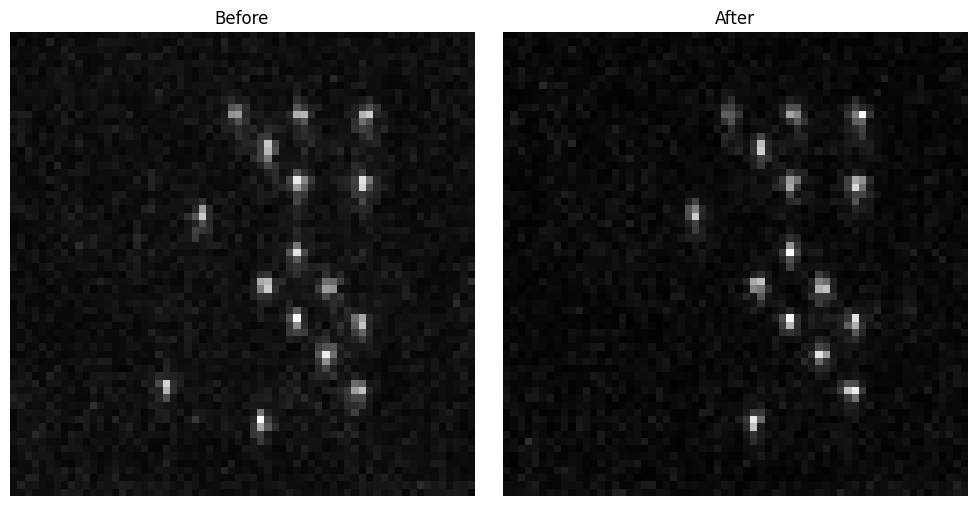
\includegraphics[width=0.78\textwidth]{assets/output1.png}
  \caption{原始 notebook 输出图 \filepath{output1.png}。教程中把它作为流程排查的参考图，而不是作为当前 run 的数据证明。}
\end{figure}


\begin{figure}[htbp]
  \centering
  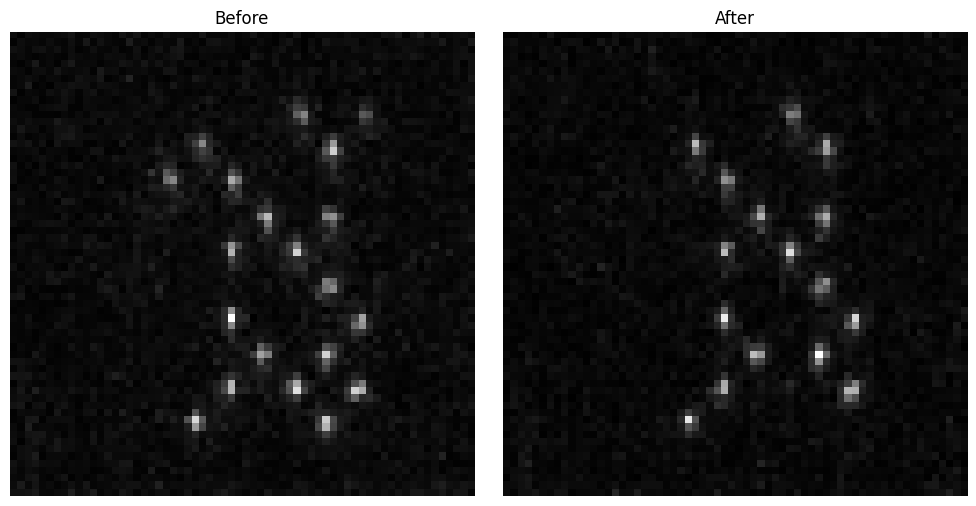
\includegraphics[width=0.78\textwidth]{assets/output2.png}
  \caption{原始 notebook 输出图 \filepath{output2.png}。教程中把它作为流程排查的参考图，而不是作为当前 run 的数据证明。}
\end{figure}


\begin{figure}[htbp]
  \centering
  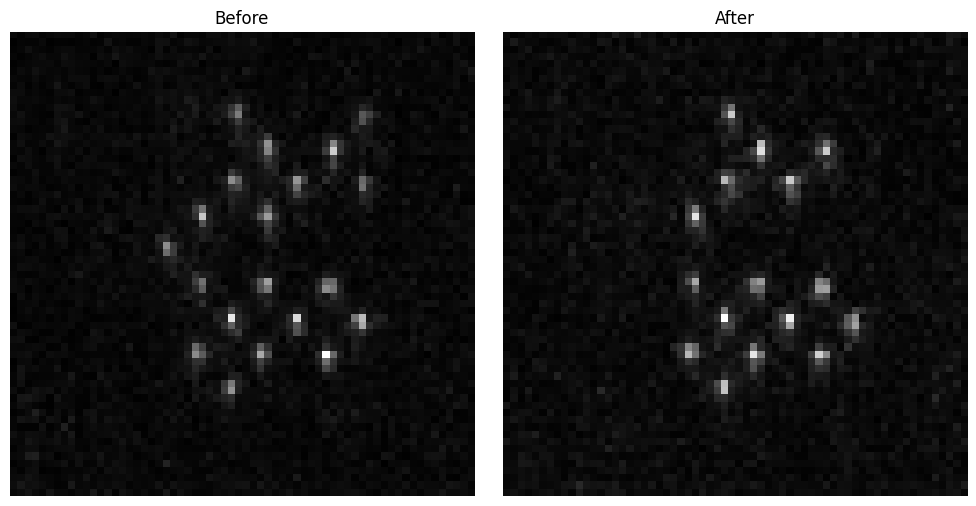
\includegraphics[width=0.78\textwidth]{assets/output3.png}
  \caption{原始 notebook 输出图 \filepath{output3.png}。教程中把它作为流程排查的参考图，而不是作为当前 run 的数据证明。}
\end{figure}


\begin{figure}[htbp]
  \centering
  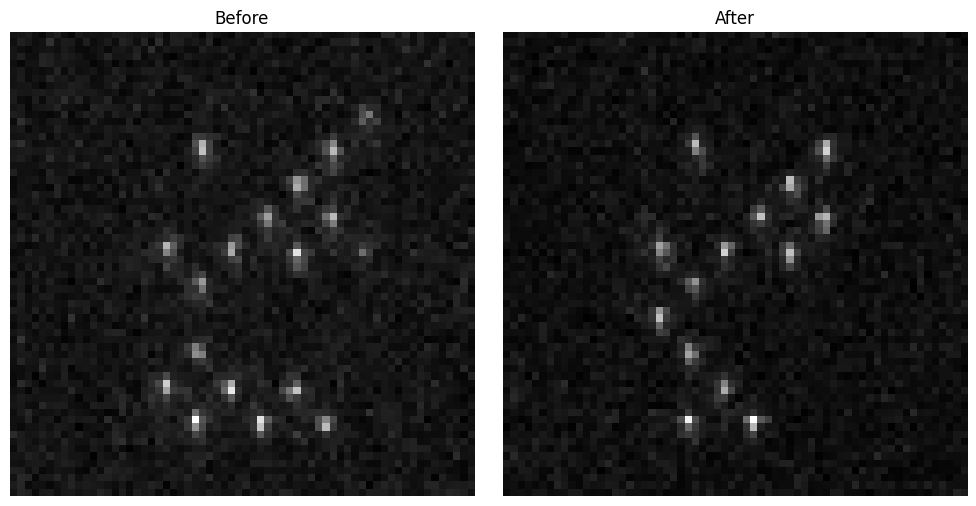
\includegraphics[width=0.78\textwidth]{assets/output11.png}
  \caption{原始 notebook 输出图 \filepath{output11.png}。教程中把它作为流程排查的参考图，而不是作为当前 run 的数据证明。}
\end{figure}


\chapter{结论}
原版 \filepath{2D_rearrangement.ipynb} 已经包含了中性原子 2D rearrangement 的全部关键思想：外触发 qCMOS 图像、loading threshold、静态阱和 AOD 频率标定、Hungarian + cascade pushing planner、PXIE RA ramp、move off、多轮成功率统计和参数扫描。它的问题不是“没有实验逻辑”，而是这些逻辑散在 notebook cell、PXIE DLL、相机外触发和手写 Verilog 时序之间，没有一个统一的 shot transaction。

最需要优先修的是 qCMOS trigger 和 FPGA/Python/PXIE 的同步边界。只要 before/after 图不再随机依赖 FPGA 自由循环，后面的 frequency map、planner 和 ramp 参数优化才有可信统计意义。否则 heatmap 再漂亮，也可能是在扫描时序抖动而不是扫描 AOD 参数。


\end{document}
